\documentclass{beamer}

\usepackage{graphicx}
\usetheme{Madrid}

\usepackage{tikz}
\usetikzlibrary{arrows.meta, positioning}

\title{Ship the changes, not the table}
\subtitle{with leech2}
\author{Lars Erik Wik}
\institute{Northern.tech}
\date{2026}

\newcommand{\blockchain}{%
\begin{center}
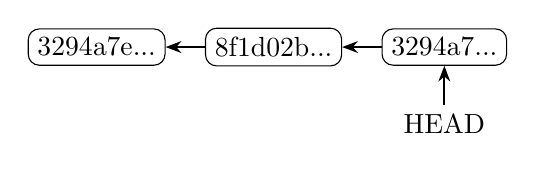
\begin{tikzpicture}[
  block/.style={draw, rounded corners},
  arr/.style={-{Stealth[length=2mm]}, thick},
]
  \node[block] (a) {3294a7e...};
  \node[block, right=5mm of a] (b) {8f1d02b...};
  \node[block, right=5mm of b] (c) {3294a7...};
  \draw[arr] (b) -- (a);
  \draw[arr] (c) -- (b);
  \node[below=5mm of c] (head) {HEAD};
  \draw[arr] (head) -- (c);
\end{tikzpicture}
\end{center}%
}

\begin{document}

\frame{\titlepage}

\begin{frame}
\frametitle{What is leech2?}
leech2 tracks changes to tables and turns them into small patches that can be applied
to a database.
\begin{itemize}
\item Computes deltas between tables and snapshots
\item Stores deltas as linked blocks
\item Consolidates blocks into a patch
\item Converts patches into SQL statements
\end{itemize}
\vfill
Written in Rust and ships with a C FFI library and a CLI tool.
\begin{block}{Documentation}
See \texttt{lch(1)} and \texttt{leech2.h(3)}.
\end{block}
\end{frame}

\begin{frame}[fragile]
\frametitle{Initializing a project}
The \texttt{lch init} command creates a work directory with a starter CSV
table and a config file telling leech2 how to interpret it.
\vfill
\begin{verbatim}
$ lch init
Initialized ./.leech2
$ ls .leech2/
config.toml  products.csv
\end{verbatim}
\end{frame}

\begin{frame}
\frametitle{The config file}
The leech2 config file can contain:
\begin{itemize}
\item Configuration options
\item Table definitions
\item Paths to drop-in fragments
\end{itemize}
\vfill
\begin{block}{Note}
Both JSON and TOML syntax is supported.
\end{block}
\end{frame}

\begin{frame}[fragile]
\frametitle{Creating the first block}
The \texttt{lch block create} command:
\begin{itemize}
\item Creates a new block
\item Records the current state
\end{itemize}
\vfill
\begin{verbatim}
$ lch block create
3294a7ec4d6f4bdb38c05fd94f0a1a8c6432f786
$ ls .leech2/state/
3294a7ec4d6f4bdb38c05fd94f0a1a8c6432f786  HEAD  STATE
\end{verbatim}
\end{frame}

\begin{frame}[fragile]
\frametitle{The block files}
Blocks are content-addressed; the name is the SHA-1 digest of the contents.
Each block contains:
\begin{itemize}
\item Reference to its predecessor
\item Creation timestamp
\item Payload
\end{itemize}
\vfill
\blockchain
\end{frame}

\begin{frame}[fragile]
\frametitle{The first block}
The first block always contains:
\begin{itemize}
\item Reference to the genesis block
\item Empty payload
\end{itemize}
\vfill
\begin{verbatim}
$ lch block show
block 3294a7ec4d6f4bdb38c05fd94f0a1a8c6432f786
Block:
  Parent: 0000000000000000000000000000000000000000
  Created: 2026-08-25 10:32:44 UTC
  Payload (0 tables)
\end{verbatim}
\end{frame}

\begin{frame}[fragile]
\frametitle{The \texttt{HEAD} file}
\texttt{HEAD} is a plain text file that points to the last block in the chain
It is updated whenever a new block is added.
\vfill
\begin{verbatim}
$ cat .leech2/state/HEAD
3294a7ec4d6f4bdb38c05fd94f0a1a8c6432f786
\end{verbatim}
\vfill
\blockchain
\end{frame}

\begin{frame}[fragile]
\frametitle{The \texttt{STATE} file}
\texttt{STATE} holds snapshots of the tables as of the most recent block.
\vfill
\begin{verbatim}
$ lch state show
State (1 tables):
  'products' [id, name, price]
    (2) "Mouse", 34.5
    (3) "Monitor", 249.95
    (1) "Keyboard", 79.99
\end{verbatim}
\vfill
\begin{block}{Note}
Primary key columns are shown in parentheses.
\end{block}
\end{frame}

\begin{frame}[fragile]
\frametitle{Creating a patch}
The \texttt{lch patch create} command consolidates the changes and stores them
in the \texttt{PATCH} file.
\vfill
\begin{verbatim}
$ lch patch create
$ ls .leech2/state/
3294a7ec4d6f4bdb38c05fd94f0a1a8c6432f786  PATCH  STATS
HEAD                                      STATE
\end{verbatim}
\vfill
\begin{block}{Note}
Performance statistics are tracked in the \texttt{STATS} file.
\end{block}
\end{frame}

\begin{frame}[fragile]
\frametitle{The \texttt{PATCH} file}
The patches contain:
\begin{itemize}
\item Reference and timestamp of the block at the head of the chain
\item Number of consolidated blocks
\item Full table contents or deltas
\end{itemize}
\vfill
\begin{block}{Note}
A patch may contain both deltas and full table contents. For each table, leech2
uses whichever is smaller.
\end{block}
\end{frame}

\begin{frame}[fragile]
\frametitle{The first patch}
The first patch contains only full table contents, since there is no earlier
state to diff against.
\vfill
\begin{verbatim}
$ lch patch show
Patch:
  Head: 3294a7ec4d6f4bdb38c05fd94f0a1a8c6432f786
  Created: 2026-08-25 10:32:44 UTC
  Blocks: 0
  States (1):
    'products' [id, name, price]
      (2) "Mouse", 34.5
      (3) "Monitor", 249.95
      (1) "Keyboard", 79.99
\end{verbatim}
\end{frame}

\begin{frame}[fragile]
\frametitle{Rendering the patch as SQL}
\texttt{lch patch sql} renders the patch as SQL statements that replicate the
changes in the database.
\vfill
\begin{verbatim}
$ lch patch sql
TRUNCATE "products";
INSERT INTO "products" ("id", "name", "price")
VALUES (2, 'Mouse', 34.5);
INSERT INTO "products" ("id", "name", "price")
VALUES (3, 'Monitor', 249.95);
INSERT INTO "products" ("id", "name", "price")
VALUES (1, 'Keyboard', 79.99);
\end{verbatim}
\end{frame}

\begin{frame}[fragile]
\frametitle{Marking the patch as applied}
\texttt{lch patch applied} records the last successful patch in the
\texttt{REPORTED} file.
\vfill
\begin{verbatim}
$ lch patch applied
3294a7ec4d6f4bdb38c05fd94f0a1a8c6432f786
$ cat .leech2/state/REPORTED
3294a7ec4d6f4bdb38c05fd94f0a1a8c6432f786
\end{verbatim}
\vfill
\begin{block}{Note}
Next patch will contain the consolidated data from \texttt{HEAD} to
\texttt{REPORTED} (exclusive).
\end{block}
\end{frame}

\begin{frame}[fragile]
\frametitle{Marking the patch as failed}
\texttt{lch patch failed} removes the \texttt{REPORTED} file, so the next patch
contains full table contents instead of deltas.
\vfill
\begin{verbatim}
$ lch patch failed --dry-run
Would have removed './.leech2/state/REPORTED'
0000000000000000000000000000000000000000
\end{verbatim}
\vfill
\begin{block}{Note}
\texttt{--dry-run} reports what would happen without changing anything.
\end{block}
\end{frame}

\begin{frame}[fragile]
\frametitle{Recording changes}
Let's change the mouse's prize from 34.50 to 29.99 and record it.
\vfill
\begin{verbatim}
$ cat .leech2/products.csv
id,name,price
1,Keyboard,79.99
2,Mouse,34.50
3,Monitor,249.95
$ sed -i 's/34\.50/29\.99/' .leech2/products.csv
$ cat .leech2/products.csv
id,name,price
1,Keyboard,79.99
2,Mouse,29.99
3,Monitor,249.95
\end{verbatim}
\end{frame}

\begin{frame}[fragile]
\frametitle{Recording changes}
\begin{verbatim}
$ lch block create
f75349613c3136219cca647565ad7c0c65051ede
$ lch block show
Block:
  Parent: 3294a7ec4d6f4bdb38c05fd94f0a1a8c6432f786
  Created: 2026-08-25 16:38:27 UTC
  Payload (1 tables):
    'products' [id, name, price]
      Updates (1):
        (2) _, 34.5 -> 29.99
\end{verbatim}
\vfill
\begin{block}{Note}
The \texttt{name} column us stripped because it's irrelevant for block
consolidation. However, the previous value of \texttt{price} is relevant.
\end{block}
\end{frame}

\begin{frame}[fragile]
\frametitle{Recording changes}
\begin{verbatim}
$ lch patch create
f75349613c3136219cca647565ad7c0c65051ede
$ lch patch show
Patch:
  Head: f75349613c3136219cca647565ad7c0c65051ede
  Created: 2026-08-25 16:38:27 UTC
  Blocks: 1
  Deltas (1):
    'products' [id, name, price]
      Updates (1):
        (2) _, 29.99
\end{verbatim}
\vfill
\begin{block}{Note}
The previous value of \texttt{price} was relevant for block consolidation, but
is not relevant for patches.
\end{block}
\end{frame}


\begin{frame}[fragile]
\frametitle{Recording changes}
Next, let's remove the monitor and record it.
\vfill
\begin{verbatim}
$ cat .leech2/products.csv
id,name,price
1,Keyboard,79.99
2,Mouse,29.99
3,Monitor,249.95
$ sed -i '/^3,/d' .leech2/products.csv
$ cat .leech2/products.csv
id,name,price
1,Keyboard,79.99
2,Mouse,29.99
\end{verbatim}
\end{frame}

\begin{frame}[fragile]
\frametitle{Recording changes}
\begin{verbatim}
$ lch block create
c4b22f2680f917bff7a61ad9f5463b52b7ee0861
$ lch block show
Block:
  Parent: f75349613c3136219cca647565ad7c0c65051ede
  Created: 2026-08-26 09:04:56 UTC
  Payload (1 tables):
    'products' [id, name, price]
      Deletes (1):
        (3) "Monitor", 249.95
\end{verbatim}
\vfill
\begin{block}{Note}
All columns are needed for block consolidation.
\end{block}
\end{frame}

\begin{frame}[fragile]
\frametitle{Recording changes}
\begin{verbatim}
$ lch patch create
c4b22f2680f917bff7a61ad9f5463b52b7ee0861
$ lch patch show
Patch:
  Head: c4b22f2680f917bff7a61ad9f5463b52b7ee0861
  Created: 2026-08-26 09:04:56 UTC
  Blocks: 2
  Deltas (1):
    'products' [id, name, price]
      Deletes (1):
        (3) _, _
      Updates (1):
        (2) _, 29.99
\end{verbatim}
\vfill
\begin{block}{Note}
Only the primary keys are relevant for patches.
\end{block}
\end{frame}

\begin{frame}[fragile]
\frametitle{Recording changes}
Execute the following queries to mirror the table on the database and mark the
patch as applied.
\vfill
\begin{verbatim}
$ lch patch sql
DELETE FROM "products"
WHERE "id" = 3;
UPDATE "products"
SET "price" = 29.99
WHERE "id" = 2;
$ lch patch applied
c4b22f2680f917bff7a61ad9f5463b52b7ee0861
\end{verbatim}
\end{frame}

\end{document}
